\section{Developing a tridiagonal solver}

\begin{frame}
\frametitle{Requirements of tridiagonal solver}

Each line of grid points yields a tridiagonal system:
\small
\begin{equation*}
 \begin{bmatrix}
     1&2\\
     1/4&1&1/4\\
     &1/4&1&1/4\\
     &&1/4&1&1/4\\
     &&&1/4&1&1/4\\
     &&&&&\ddots\\
     &&&&&&\ddots\\
     &&&&&&&\ddots\\
     &&&&&&&2&1
  \end{bmatrix}
  \begin{bmatrix}
      f^{\prime}_1 \\
      f^{\prime}_2 \\
      f^{\prime}_3 \\
      \vdots \\
      \vdots \\
      \vdots \\
      \vdots \\
      f^{\prime}_{n-1} \\
      f^{\prime}_n
   \end{bmatrix}
 =
 \begin{bmatrix}
     \frac{-5f_1 + 4f_2 + f_3}{2dx}\\
     \frac{3(f_{3} - f_{1})}{4dx}\\
     \frac{3(f_{4} - f_{2})}{4dx}\\
     \vdots\\
     \vdots\\
     \vdots\\
     \vdots\\
     \frac{3(f_{n} - f_{n-2})}{4dx}\\
     \frac{5f_{n} - 4f_{n-1} - f_{n-2}}{2dx}
  \end{bmatrix}
\end{equation*}
\end{frame}

\begin{frame}
\frametitle{Requirements of tridiagonal solver}
\begin{columns}
\begin{column}{0.5\textwidth}
\begin{itemize}
\item For a 1-D grid, solution gives the derivative
    at all points simultaneously
\item For 2-D and 3-D grids, we solve a tridiagonal system
    for each grid line
\item The coefficient matrix is the same for each system
\item Only right hand sides are different
\end{itemize}
\end{column}
\begin{column}{0.5\textwidth}
    \hspace{1cm}
    \includegraphics[width=100px]{img/grid-lines.eps}
\end{column}
\end{columns}
\end{frame}

\begin{frame}
\frametitle{Thomas algorithm}
\begin{itemize}
\item Derived from Gaussian elimination
\item Requires $2n$ steps and $4n$ storage
\item The most efficient serial implementation
\item What about for GPUs?
    \begin{itemize}
        \item inherently sequential
        \item can use multiple threads to solve
            individual tridiagonal systems
    \end{itemize}
\end{itemize}
\end{frame}

\begin{frame}
\frametitle{Issues with GPU implementation}
\begin{columns}
\begin{column}{0.5\textwidth}
\begin{itemize}
    \item Uncoalesced global memory accesses
    \item What about shared memory?
        \begin{itemize}
            \item 4N storage \emph{per block}
            \item SM shared memory filled up quickly
            \item very few threads per SM
            \item under-utilizes the GPU parallelism
        \end{itemize}
    \item $2n$ steps - can do better on GPU
\end{itemize}
\end{column}
\begin{column}{0.5\textwidth}
    \includegraphics[width=150px]{img/pThomas.eps}
\end{column}
\end{columns}
\end{frame}

\begin{frame}
\frametitle{Tridiagonal solvers for the GPU}
\begin{itemize}
\item Zhang et al. (2010) describe the implementation
    of three algorithms for tridiagonal systems on GPUs
    \begin{itemize}
        \item Cyclic reduction
        \item Parallel cyclic reduction
        \item Recursive doubling
    \end{itemize}
\item Exhibit \emph{fine-grained} parallelism
\item Subsequent efforts based on CR and PCR primarily
\end{itemize}
\end{frame}

\begin{frame}
\frametitle{Cyclic reduction}
\begin{columns}
\begin{column}{0.5\textwidth}
\begin{itemize}
\item Buzbee and Goleb (1970)
\item \textbf{Forward reduction} ($log(n)-1$ steps):
    \begin{itemize}
    \item Eliminate odd-indexed equations at each step
    \item Two-by-two system is left
    \end{itemize}
\item \textbf{Backward substitution} ($log(n)-1$ steps):
    \begin{itemize}
    \item Solve for odd-indexed equations using even-indexed values
    \end{itemize}
\item Best case ($n$ parallel threads): requires $2log(n)-1$ steps
\end{itemize}
\end{column}
\begin{column}{0.5\textwidth}
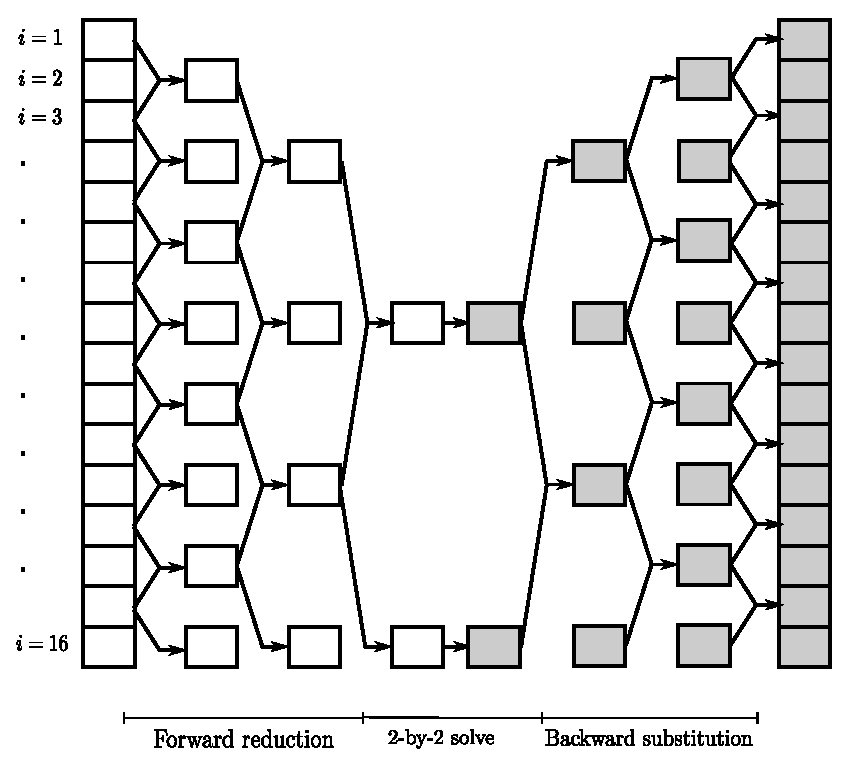
\includegraphics[width=150px]{img/cyclic-reduction.eps}
\end{column}
\end{columns}
\end{frame}

\begin{frame}
\frametitle{GPU implementation}
\begin{columns}
\begin{column}{0.5\textwidth}
\begin{itemize}
\item Each tridiagonal system mapped to a thread block;
    individual threads mapped to equations
\item Several systems can be solved at concurrently
\item Forward reduction: diagonal arrays $a$, $b$, $c$ and RHS $d$
    updated \emph{in-place}
\item Backward substitution: solution $x$ computed
    from $a^\prime$, $b^\prime$, $c^\prime$ and $d^\prime$
\item Synchronization required at each step
\end{itemize}
\end{column}
\begin{column}{0.5\textwidth}
\only<1>{
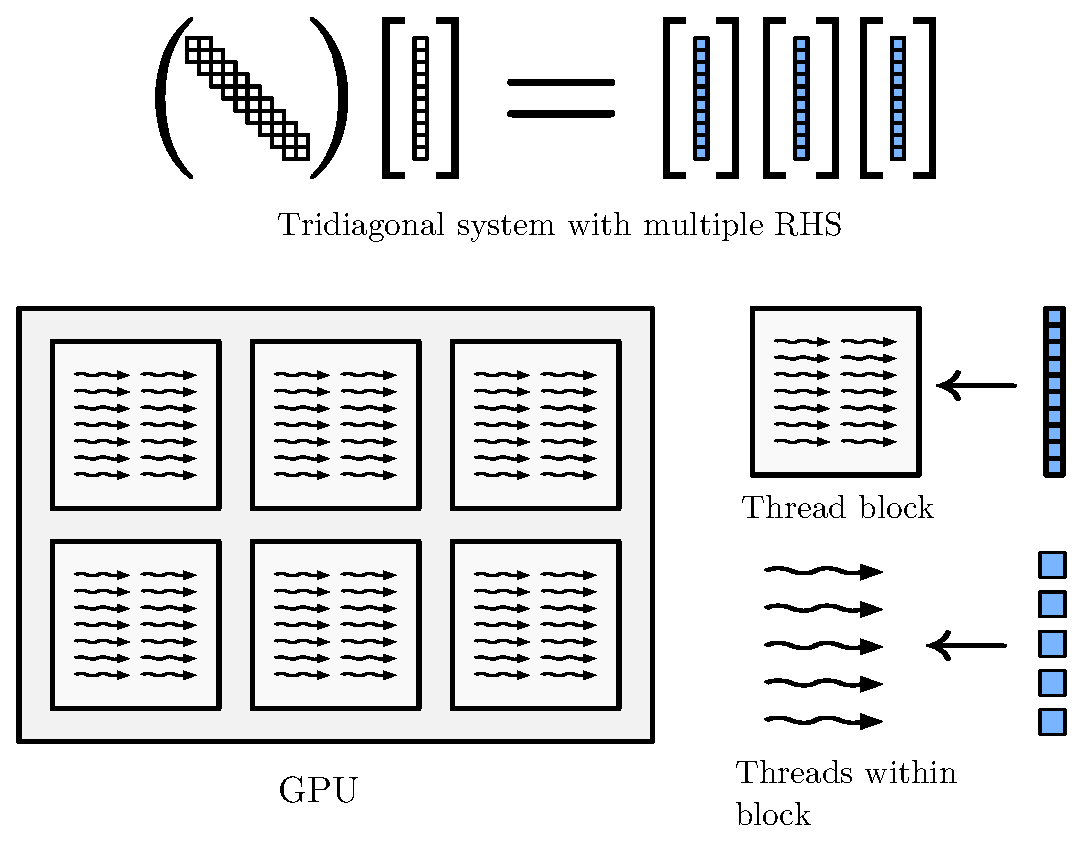
\includegraphics[width=150px]{img/gpu-mapping.eps}
}
\only<2>{
\centering
Forward reduction
\scalebox{0.8}{
\vbox{
\begin{align*} 
    k_1 &= \frac{a_i}{b_{i-1}}, k_2 = \frac{c_i}{b_{i+1}} \\
    a^{\prime}_i &= -a_{i-1}k_1 \\
    b^{\prime}_i &= b_i - c_{i-1}k_1 - a_{i+1}k_2 \\
    c^{\prime}_i &= -c_{i+1}k_2 \\
    d^{\prime}_i &= d_i - d_{i-1}k_1  - d_{i+1}k_2 \\
\end{align*}}}

\centering
Backward substitution
\scalebox{0.8}{
\vbox{
\begin{align*}
x_i &= \frac{d^{\prime}_i - a^{\prime}_ix_{i-1} - \
    c^{\prime}_ix_{i+1}}{b^{\prime}_i}
\end{align*}}}}

\end{column}
\end{columns}
\end{frame}

\begin{frame}
\frametitle{Issues}
\begin{columns}
\begin{column}{0.5\textwidth}
\begin{itemize}
    \item Thread activity
    \item Uncoalesced global memory access
    \item Bank conflicts
    \item Limited shared memory
\end{itemize}
\end{column}
\begin{column}{0.5\textwidth}
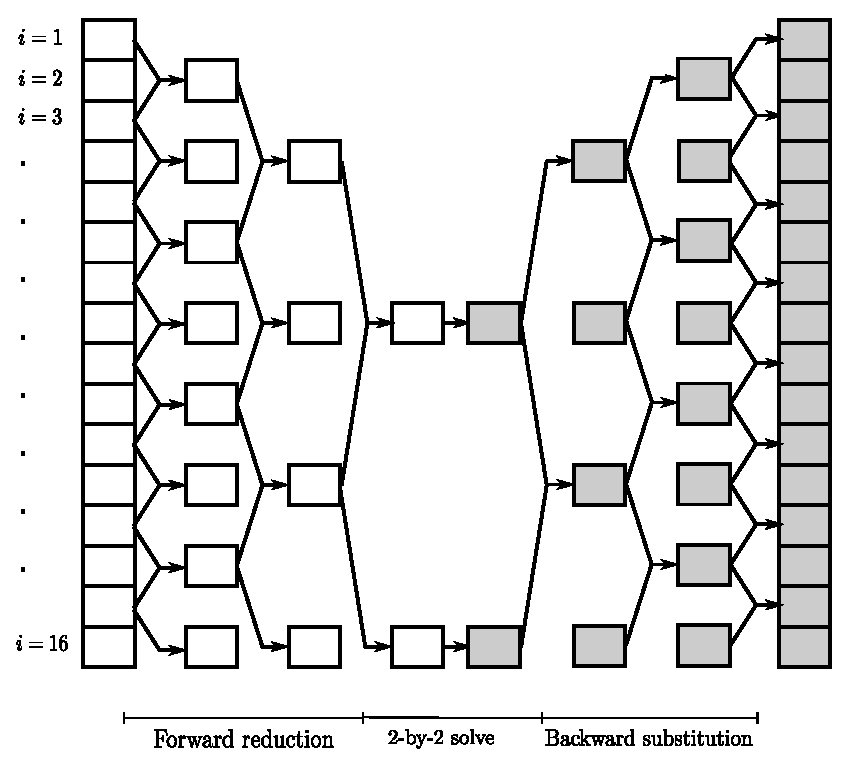
\includegraphics[width=150px]{img/cyclic-reduction.eps}
\end{column}
\end{columns}
\end{frame}

\begin{frame}
\frametitle{Efforts for improving performance}
\begin{itemize}
    \item Zhang et al.: hybrid CR+PCR solver
    \item G{\"o}ddeke et al.: separate even and odd indexed
        coefficients
    \item Davidson et al.: register packing
    \item Esfahanian et al.: global memory with data rearrangement
\end{itemize}
\end{frame}

\begin{frame}
\frametitle{A novel approach}
\begin{itemize}
\item Solving systems with same RHS
\item Computing $a^\prime$, $b^\prime$ and $c^\prime$
    for each system and at every time step - redundant
\item Storing coefficients (similar to LU) - expensive
\item The coefficient matrix has relatively simple structure
\item Can be exploited to improve cyclic reduction performance
\end{itemize}
\end{frame}

\begin{frame}
\begin{columns}
\begin{column}{0.5\textwidth}
\begin{itemize}
    \item Diagonals are nearly constant (\emph{near-Toeplitz})
    \item Symmetry may be broken by boundary conditions
    \item Near-Toeplitz matrices occur in other numerical schemes
    \begin{itemize}
        \item Alternating direct implicit methods
        \item Line relaxation methods
        \item Poisson solvers
        \item One-dimensional ODEs and PDEs
    \end{itemize}
\end{itemize}
\end{column}
\begin{column}{0.5\textwidth}
\centering
\scalebox{0.6}{%
\vbox{
\begin{equation*}
\begin{bmatrix}
     1&2\\
     1/4&1&1/4\\
     &1/4&1&1/4\\
     &&1/4&1&1/4\\
     &&&1/4&1&1/4\\
     &&&&&\ddots\\
     &&&&&&\ddots\\
     &&&&&&&\ddots\\
     &&&&&&&2&1
  \end{bmatrix}
\end{equation*}}}
\end{column}
\end{columns}
\end{frame}

\begin{frame}
\frametitle{General approach}
\begin{columns}
\begin{column}{0.5\textwidth}
\begin{itemize}
\item {First reduction step: substitute:
    \scalebox{0.8}{
    \vbox{
    \begin{align*}
        a_2 &= a_3 = a_4 = \hdots &\equiv a_0 \\
        b_2 &= b_3 = b_4 = \hdots &\equiv b_0 \\
        c_2 &= c_3 = c_4 = \hdots &\equiv c_0
    \end{align*}}}}
\item $a^\prime$, $b^\prime$, $c^\prime$
    represent coefficients of the ``reduced'' tridiagonal system
\item \textbf{The reduced system is also near-Toeplitz}
\item Each forward reduction step produces a near-Toeplitz
    tridiagonal system
\item Coefficients can be stored compactly
\end{itemize}
\end{column}
\begin{column}{0.5\textwidth}
\centering
Forward reduction
\scalebox{0.8}{
\vbox{
\begin{align*} 
    k_1 &= \frac{a_i}{b_{i-1}}, k_2 = \frac{c_i}{b_{i+1}} \\
    a^{\prime}_i &= -a_{i-1}k_1 \\
    b^{\prime}_i &= b_i - c_{i-1}k_1 - a_{i+1}k_2 \\
    c^{\prime}_i &= -c_{i+1}k_2 \\
    d^{\prime}_i &= d_i - d_{i-1}k_1  - d_{i+1}k_2 \\
\end{align*}}}
\end{column}
\end{columns}
\end{frame}

\begin{frame}
Cyclic reduction reduced to:

\vspace{1cm}

\textbf{Forward reduction}
\begin{align*}
d^{\prime}_i = d_i - d_{i-1}k_1^{m}  - d_{i+1}k_2^{m}
\end{align*}

\textbf{Backward substitution}
\begin{align*}
x_i = \frac{d^{\prime}_i - a^mx_{i-1} - \
    c^{m}x_{i+1}}{b^m}
\end{align*}

where $a^m$, $b^m$ and $c^m$ are the precomputed
coefficients for $i>1$ at the step $m$.
\end{frame}
